\section{研究背景及意义}

随着互联网技术的发展,越来越多的数据不再存储在本地设备上,而是托管在服务器中,用户只需在使用时向服务器请求数据,从而极大地拓展了数据的可用性和易用性。然而,这种便利性也带来了一个问题:用户的访问模式可能会泄露他们的隐私。以DNS查询为例,用户的DNS请求会暴露他们正访问的域名。另一个例子是密码泄露查询服务,如图\ref{fig:password-query}所示,用户提供密码后,服务会告知用户该密码是否曾在以往的数据泄露中出现过。如果用户以明文密码直接进行查询,就会将密码泄露给服务提供者。在更为敏感的领域,如军工、政府和医疗行业,这些泄露更难以接受。如此看来,现代互联网的数据使用逻辑要求我们以更安全的方式访问数据。

\begin{figure}
    \centering
    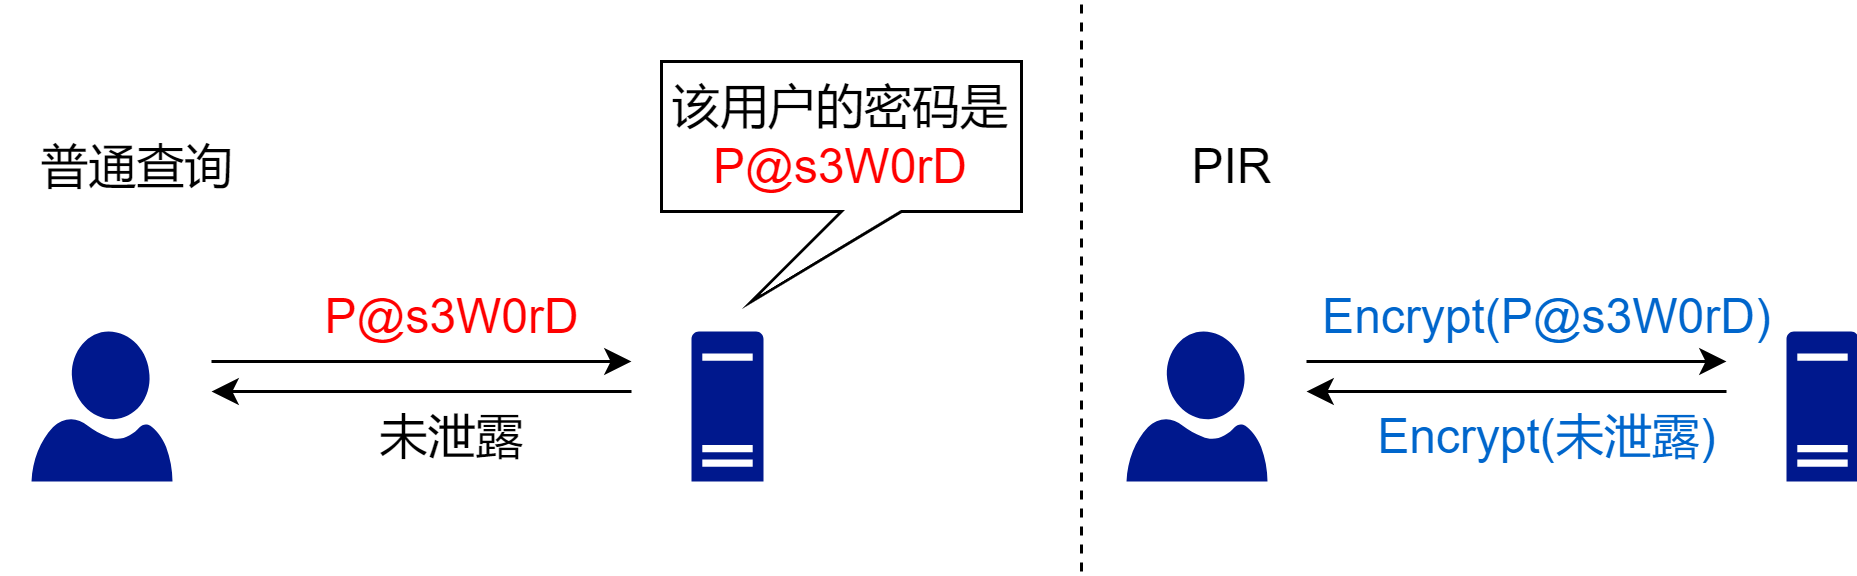
\includegraphics[width=0.8\textwidth]{figure/密码查询服务.png}
    \caption{密码泄露查询服务}
    \label{fig:password-query}
\end{figure}

密码学领域针对这一问题提出了隐匿查询(Private Information Retrieval,PIR)这一原语。PIR技术允许数据请求方发起加密的请求:如图\ref{fig:password-query}中右图所示,用户请求服务器中的数据,但不泄露具体请求的是哪一条数据。实际操作中,客户端通常会向服务器发送一个加密的查询索引,服务器根据协议对查询索引与数据库进行计算,然后将结果反馈给客户端,客户端再将加密结果解密为相应数据。这一原语有效地避免了用户访问内容的泄露,为DNS查询、密码泄露查询等多种敏感服务提供了潜在的解决方案。

然而,PIR技术也存在一些局限性。首先,相较于普通的数据库查询,PIR的效率要低得多:PIR涉及大量的计算和通信。在大多数PIR协议中,服务器需要遍历整个数据库才能完成一次查询。当前最先进的单服务器PIR协议可达到约10GiB/s的数据吞吐量,这意味着在40GiB大小的数据库中进行一次查询至少需要4秒。因此,现实中PIR技术仅适用于较小规模的数据库。其次,PIR无法有效利用传统数据库中的索引功能,这通常导致服务器需要将整个数据库加载到内存中。这无疑提高了PIR对硬件的要求,对服务器的内存容量提出了挑战。自1995年PIR被提出以来 \cite{FOCS:CGKS95},该技术经历了多年的发展,但对于许多应用场景而言,目前的PIR协议仍在成本上显得过于昂贵,因此缺少大规模应用案例。

从另一个角度来看,人们逐渐认识到在线服务的可靠性和准确性极为必要。当我们将数据交付给云服务器供他人查询时,必须采取措施以确保查询结果的准确性和服务的可用性。半数时间宕机、剩下时间出错的服务毫无意义。在科研、军事、医疗等领域,可靠性和准确性更是必须满足的要求,网络波动、硬件错误、恶意攻击所导致的错误都可能引发严重后果。特别是在零信任的环境下,区块链、DePIN等去中心化基础设施模型对可靠性提出了更高的要求。为了将PIR应用于更广泛领域,迫切需要支持可验证且高可用的PIR协议。

本文提出了一套适用于区块链的PIR协议和应用框架,目的在于(i) 降低PIR服务的计算负担 (ii) 验证查询结果 (iii) 减轻服务器存储压力,提高可用性,以此拓展PIR的实际应用范围。